\chapter{Conclusion}
\section{Results}
In the preliminary game with the other team, we lose the game of 2:3, as our striker are not working properly. After a long time tuning and testing, we fixed the existing problems for calibration and localization and implemented our new behavior for the defender and striker. As a result, in the last game on the presentation day, our yellow team beat the other team with 2:0.
\section{Suggestion for the future work}
Although there are already some nice improvement this semester, more work need to be done in the future to get better performance. Here are two main ideas for the role behavior improvement for the future:
\begin{itemize}
    \item Dynamic role assignment
    \item ``Intelligent'' choice of kick direction
\end{itemize}
\subsection{Dynamic role assignment}
The situation of a real game changes really fast. To achieve better result, the dynamic role assignment needs to be implemented. More concretely, the robots will decide by himself which role he is playing. If the position of the defender is over the supporter, their roles could be exchanged immediately. So the original defender don't need to wasting time going back and the original supporter don't need to going forward again to keep their ``set'' behavior. In addition, if the supporter is ahead of striker by some reason, he should automatically work as the striker as in that situation he can score easier.
With this improvement, the team will work more efficiently and more dynamic strategies can be found.
\subsection{``Intelligent'' choice of kick direction}
The proposed method in Section~\ref{sec:Striker} is already a nice improvement over the original kick direction. But if the opponent goal-keeper react quickly and strongly enough, he may still be able to stop it. As shown in \fref{fig:IntKik}, the direction of the kicking should be determined by calculating the distance of the goalkeeper to different goal posts(marked with red dotted lines). If the goalkeeper is near to the left post like the shown graph, the kicking direction should be the right goal post. With this method the goalkeeper will not be able to stop the ball as he is already too far away from the other goal post.
\begin{figure}[!htb]
    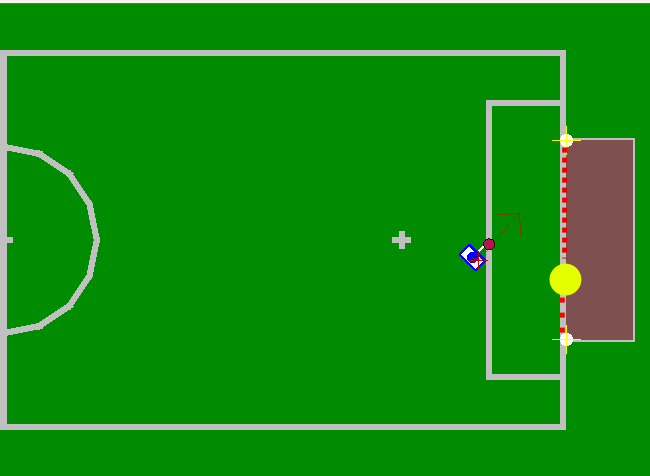
\includegraphics[scale = 0.3]{pics/striker_future}
    \centering
    \caption{``Intelligent'' choice of kick direction}
    \label{fig:IntKik}
\end{figure}
